\section{5G Ecosystem}
{As a leader in 5G technology, Huawei has completed inter-operability development testing (IODT) with mainstream chip, terminal, and network vendors. Huawei became the first company worldwide to launch the industry-first 5G commercial chip with 3GPP release 15. Huawei are the only vendor who can provide end-to end commercial solutions, vigorously promoting the maturity and commercial use of the 5G industry chain.}

\begin{figure}
    \centering
    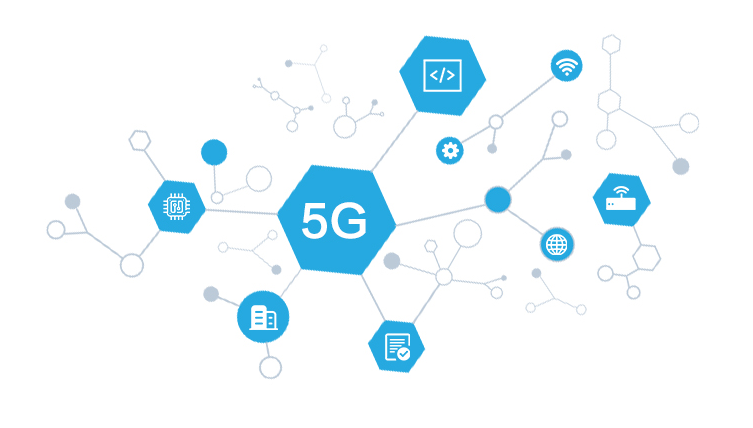
\includegraphics[width=11cm]{Images/lastimg.png}
    \caption{5G Ecosystem}
    \label{fig:my_label}
\end{figure}

\section{The Approach}
\subsubsection{Imagining the mobile services of the next decade.}

{As with each preceding generation, the rate of adoption of 5G and the ability of operators to monetize it will be a direct function of the new and unique use cases it unlocks. Thus, the key questions around 5G for operators are essentially\\ \item a. What could users do on a network which meets the 5G requirements listed above that is not currently possible on an already existing network?\\  \item b. How could these potential services be profitable?\\

\item These technologies have a number of potential use cases in both entertainment (e.g., gaming) and also more practical scenarios such as manufacturing or medicine and could extend to many wearable technologies. For example, an operation could be performed by a robot that is remotely controlled by a surgeon on the other side of the world. This type of application would require both high bandwidth and low latency beyond the capabilities of LTE, and therefore has the potential to be a key business model for 5G networks.\\ 

\item However, it should be pointed out that VR/AR systems are very much in their infancy and their development will be largely dependent on advances in a host of other technologies such as motion sensors and heads-up display (HUD). It remains to be seen whether these applications could become profitable businesses for operators in the future\\}

\subsubsection{Autonomous Driving/Connected Cars}

Enabling vehicles to communicate with the outside world could result in considerably more efficient and safer use of existing road infrastructure. If all of the vehicles on a road were connected to a network incorporating a traffic management system, they could potentially travel at much higher speeds and within greater proximity of each other without risk of accident - with fully-autonomous cars further reducing the potential for human error. While such systems would not require high bandwidth, providing data with a command-response time close to zero would be crucial for their safe operation, and thus such applications clearly require the 1 millisecond delay time provided in the 5G specification. In addition, a fully ‘driverless’ car would need to be driverless in all geographies, and hence would require full road network coverage with 100 percent reliability to be a viable proposition.

\subsubsection{Wireless Cloud-Based Office/Multi-Person Videoconferencing}

High bandwidth data networks have the potential to make the concept of a wireless cloud office a reality, with vast amounts of data storage capacity sufficient to make such systems ubiquitous. However, these applications are already in existence and their requirements are being met by existing 4G networks. While demand for cloud services will only increase, as now they will not require particularly low latencies and therefore can continue to be provided by current technologies or those already in development. While multi-person video calling - another potential business application - has a requirement for lower latency, this can likely be met by existing 4G technology.

\subsection{Machine-to-Machine Connectivity (M2M)}
M2M is already used in a vast range of applications but the possibilities for its usage are almost endless. Our forecasts predict that the number of cellular M2M connections worldwide will grow from 250 million this year to between 1 and 2 billion by 2020, dependent on the extent to which the industry and its regulators are able to establish the necessary frameworks to fully take advantage of the cellular M2M opportunity. Typical M2M applications can be found in ‘connected home’ systems (e.g., smart meters, smart thermostats, smoke detectors), vehicle telemetries systems (a field which overlaps with Connected Cars above), consumer electronics and health-care monitoring. Yet the vast majority of M2M systems transmit very low levels of data and the data transmitted is seldom time-critical. Many currently operate on 2G networks or can be integrated with the IP Multimedia Subsystem (IMS) – so at present the business case for M2M that can be attached to 5G is not immediately obvious.

\subsubsectionA True Requirement for a Generational Shift?}
Thus, many of the services that have been put forward as potential ‘killer apps’ for 5G do not require a generational shift in technology and could be provided via existing network technologies. Only applications that require at least one of the key 5G technical requirements –sub-1ms latency and Gbps downlink speed – can be considered true next generational business cases.\item Of these two requirements, reducing latency to sub-1ms levels may provide the greatest technical challenge. Meanwhile, operators are already making a considerable amount of progress in increasing the data speeds of their existing networks by adopting LTE-A \item technologies. While it is important to note that although many of the use cases and services discussed in this section do not strictly require 5G, they could offer an enhanced user experience on a 5G network. However, this amounts to an incremental benefit that is more difficult to market than a genuine new service, and not a core component of any 5G business case.

% \begin{figure}
%     \centering
%     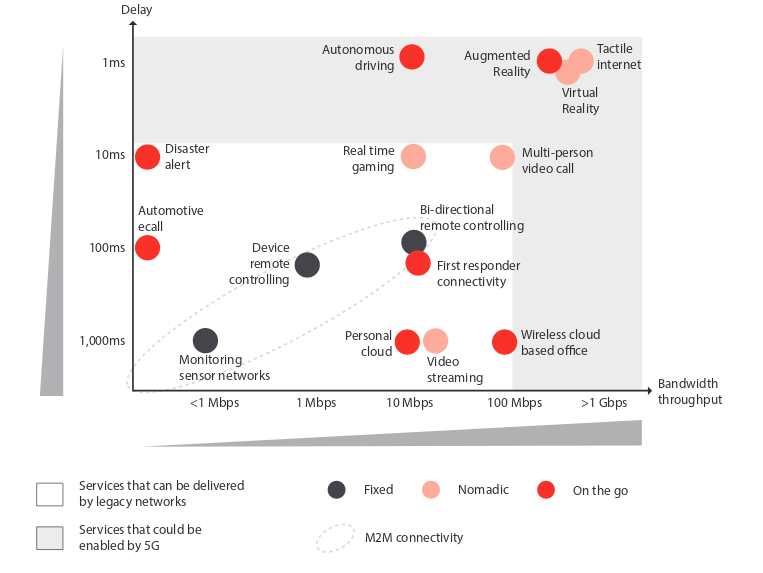
\includegraphics[width=6cm]{Images/prespective.png}
%     \caption{Caption}
%     \label{fig:my_label}
% \end{figure}